\section{Methods and Material}
%%\fxnote{Write something about what we're comparing with, the codes we're
%%using, and how we set up the simulations.}


To resolve well-known computational aerodynamics and aeroelastic airfoils, a coupled FSI solver is combined with the turbulence model k-$\omega$ SST and large deformation updated Lagrangian finite volume structure solver \cite{Cardiff2014AOrientations}. As a first step for the ongoing numerical simulations, the validations based on NACA6409 are performed and compared to the results of previous experiments \cite{Gamble2020a}.


%\subsection{Model}

The previous work of \citet{Gamble2020b} considered the modelling of feather-like airfoil as two part segments: rigid part and flexible one (Fig. \ref{fig:segments}). The rachis' structure mimics that of a narrow cavity in general, with a circular cross section at the root and a rectangular cross section at the trailing edge.

\citet{Bachmann2012FlexuralProperties} provided in various biological experiment on the rachis, different material properties such as the Young's modulus $\mathcal{E}$ (Modulus of elasticity).

Following the work of \cite{Gamble2020a}, we use simplified bird airfoil as the basis for this computational study and a Young's modulus $\mathcal{E}$ of both 2.5GPa and  689.5MPa chordwise stiffness that may allow feather replication with a canstant Young’s modulus,though the Ref \cite{Gamble2020b} used a $\mathcal{E}$ variable ranging [2.5-0.5 GPa] in stiffness characteristics towards the tip of the feather’s trailing edge.

Airfoil configuration and computational mesh used for the fluid–solid interaction problem is shown in Figure \ref{fig:Ggeometry}. As shown in Figure \ref{fig:Griddomain}, the computational domain is built with a structured grid using the ANSYS multi-blocks grid ICEM tool, with the appropriate boundary conditions. The mesh plane is extruded in span wise direction with a one cell.
FSI Simulations are perfomed with an open-source finite volume toolbox for solid mechanics and fluid-solid interaction simulations. The finite volume method described in \citet{Cardiff2018} for orthotropic bodies subjected to large strains and large deformations with consideration of updated Lagrangian finite volume solver \cite{Tukovic2014} is implemented in the FSI method described in this work. 

\begin{figure}[hbt!]
  \centering
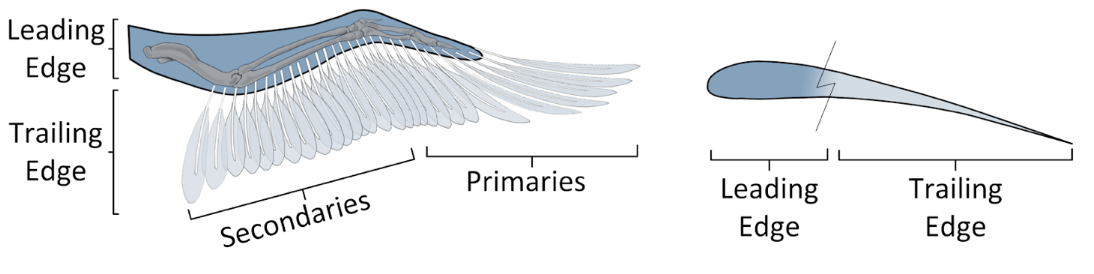
\includegraphics[width=4in]{Figures/gamble inman.png}
\caption{\label{fig:segments} Anatomy of bird airfoil considering rigid and flexible segments \cite{Gamble2020a}}
\end{figure}

The next section \ref{sec:preliminary} outlines the preliminary resulting data assessed in multiple stages of the study of the NACA6409 airfoil (Fig.\ref{fig:6409}) at Re ($10^5$–5x$10^5$) considering a rigid segment of 40\% and flexible segment 60\% chord length (Fig. \ref{fig:airfoilSegments}). In addition, it identifies avenues for further assessment of the man-made-bird-like AS6095 airfoil (Fig.\ref{fig:AS6095}) designed by \citet{Ananda2018a} at moderate low Reynolds number of $10^5$. Further,  a case study investigates the flow behavior for the known owl-like airfoil (Fig.\ref{fig:owl}) operating at very low Reynolds of $2.3\times 10^4$.

\begin{figure}[hbt!]
  \centering
\begin{subfigure}{.4\textwidth}
   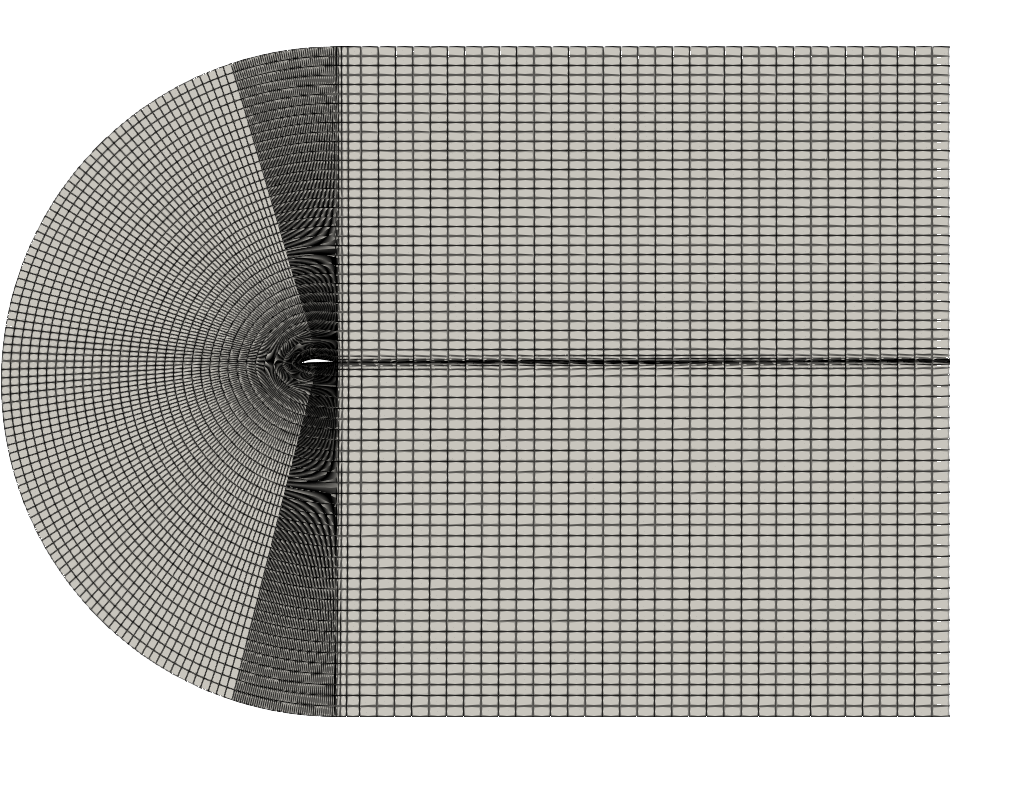
\includegraphics[width=2.8in]{Figures/mesh fluid.png}
%   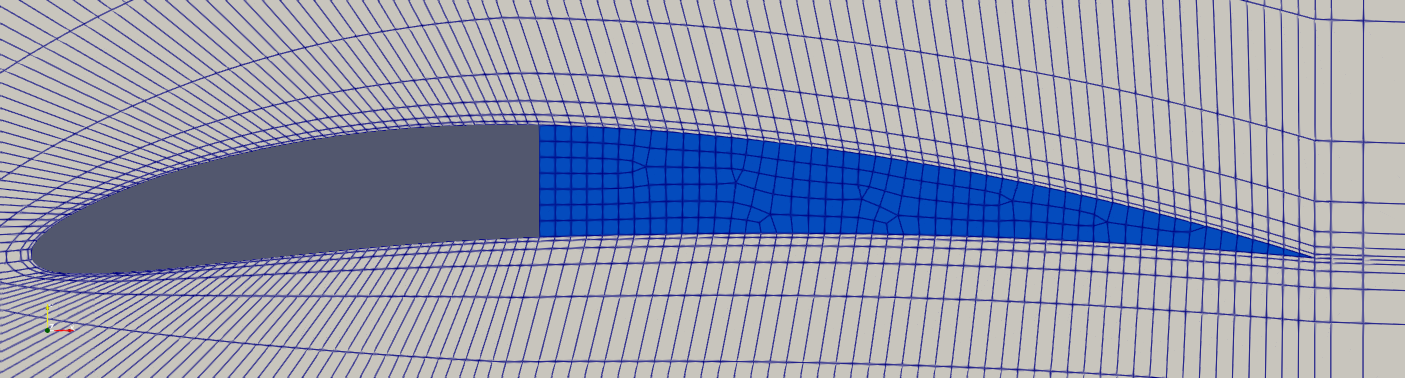
\includegraphics[width=3in]{Figures/mesh solid.png}
  \caption{\label{fig:Griddomain} Grid domain}
\label{fig:airfoildesigna}
\end{subfigure}
\begin{subfigure}{.4\textwidth}
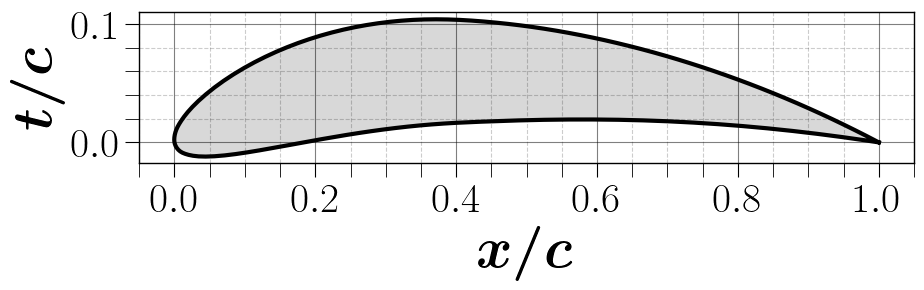
\includegraphics[width=.6\columnwidth]{Figures/naca_airfoil.png}
\caption{\label{fig:6409}NACA6409}
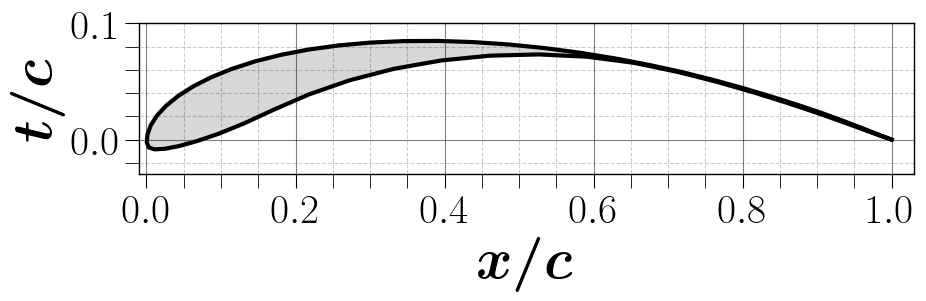
\includegraphics[width=.6\columnwidth]{Figures/AS9065_airfoil.png}
\caption{\label{fig:AS6095}AS6095 airfoil \cite{Ananda2018}}
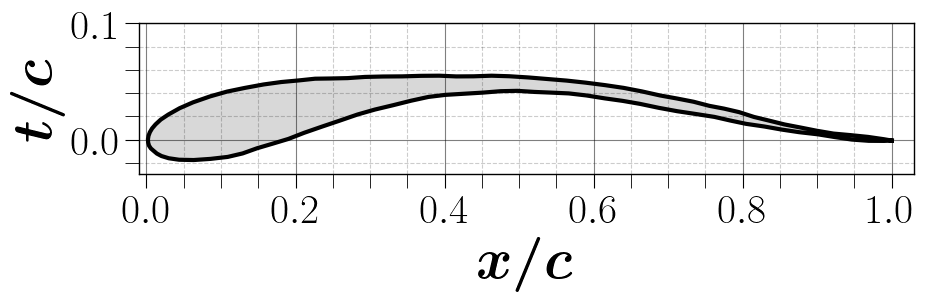
\includegraphics[width=.6\columnwidth]{Figures/owl_airfoil.png}
\caption{\label{fig:owl}Owl airfoil \cite{Liu2004}}
\end{subfigure}
\caption{\label{fig:Ggeometry} Computational domain and airfoil profiles}
\end{figure}

\begin{figure}[hbt!]
  \centering
   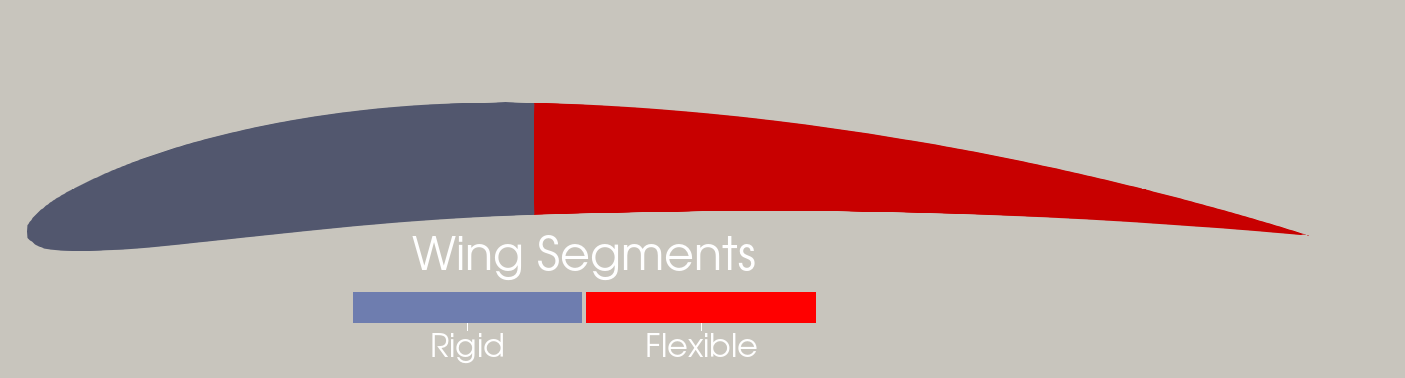
\includegraphics[width=3in]{Figures/airfoilgeometry.png}
  \caption{\label{fig:airfoilSegments} NACA6409 airfoil segments (40\% ) rigid and (60\%) flexible denoted $\mathcal{L}$}
\end{figure}

%\subsection{Materials Properties}
%\begin{table}[hbt!]
%\caption{\label{tab:materproper} Material properties}
%\centering
%\begin{tabular}{ccccc}
%  \hline
%  Material & scientific name & Young Modulus & stiffness\\
%  \hline
%  rubber       & 10 m/s           & 0.0005 m       & -1.40 K/hr\\
%  rachis       & Keratin          & 689.5MPa       & -1.50 K/hr \\
%\hline
%\end{tabular}
%\end{table}
%\subsection{Methods}
%\footnote{\url{https://bitbucket.org/philip_cardiff/solids4foam-release}}
%\subsection{Computational methodology and Validation}
